\documentclass[man,apacite,floatsintext]{apa6}

\usepackage{graphicx}
\usepackage[utf8]{inputenc}
\usepackage{todonotes}

\title{Much ado about acquiesence}
\shorttitle{Acquiesence and validity}

\twoauthors{Yphtach Lelkes}{Rebecca Weiss}
\twoaffiliations{University of Amsterdam}{Stanford University}
\abstract{This is an example of a journal article using the \texttt{apa6.cls} document class to typeset manuscripts according to 6th edition of the Americal Psychological Association (APA) manual}
\rightheader{APA style}
\leftheader{Author One}


\begin{document}

\maketitle

\section{Methods}

Data came from the ANES 2012 Time Series study. The two-wave pre- and post-election study combines online and face-to-face interviews, and yielded a total sample of 5,916 interviews in the pre-election wave (2,056 face-to-face and 3,860 online) and 5,513 interviews in the post-election wave. 

\subsection{Target Measures} 
Respondents were randomly assigned to receive either the agree-disagree form or the construct-specific form of a set of four items designed to measure political efficacy. Respondents that saw one set of items in the pre-election wave, saw the same set of items in the post election wave. 
\todo{We can probably put a ton of this in the appendix}
\paragraph{Agree-Disagree Battery}
For each of the following statements, respondents were asked, ``Do you AGREE STRONGLY, AGREE SOMEWHAT, NEITHER AGREE NOR DISAGREE, DISAGREE SOMEWHAT, or DISAGREE STRONGLY with this statement?''
\begin{itemize}
\item Efficacy 1:  ``Sometimes, politics and government seem so complicated that a person like me can't really understand what's going on.''
\item Efficacy 2:  ``I feel that I have a pretty good understanding of the important political issues facing our country.''
\item Efficacy 3: ``Public officials don't care much what people like me think.''
\item Efficacy 4: ``People like me don't have any say about what the government does.''
\end{itemize}

\paragraph{Construct-Specific Battery}
\begin{itemize}
\item Efficacy 1: ``How often do politics and government seem so complicated that you can't really understand what's going on?'' [ALWAYS, MOST OF THE TIME, ABOUT HALF THE TIME, SOME OF THE TIME, or NEVER] 
\item Efficacy 2: ``How well do you understand the important political issues facing our country?'' [EXTREMELY WELL, VERY WELL, MODERATELY WELL, SLIGHTLY WELL, or NOT WELL AT ALL]
\item Efficacy 3: ``How much do public officials care what people like you think?'' [A GREAT DEAL, A LOT, A MODERATE AMOUNT, A LITTLE, or NOT AT ALL]
\item Efficacy 4: ``How much can people like you affect what the government does?'' [A GREAT DEAL, A LOT, A MODERATE AMOUNT, A LITTLE, or NOT AT ALL]
\end{itemize}

\subsection{Criterion Measures} We chose criterion items that have been shown to be correlated with the core constructs (internal efficacy and external efficacy) but do not share the response scale of the of either set of target items. This was to ensure that criterion and target item correlations were not artifacts of a similar response scale. Three indicators, all relating to political activism (the outcome measure in most political efficacy studies), met these requirements. 

\paragraph{Political Activities}
The ANES asked respondents whether they had or had not done each of the following political activities in the past 4 years:

\begin{itemize}
\item ``...joined in a protest march, rally, or demonstration''
\item ``...you attended a meeting of a town or city government or school board''
\item ``...signed a petition on the Internet about a political or social issue''
\item ``...signed a petition on paper about a political or social issue''
\item ``...given money to a religious organization''
\item ``...given money to any other organization concerned with a political or social issue''
\item ``...called a radio or TV show about a political issue''
\item ``...sent a message on Facebook or Twitter about a political issue''
\item ``...written a letter to a newspaper or magazine about a political issue''
\item ``...contacted or tried to contact a member of the U.S. Senate or U.S. House of Representatives''
\end{itemize}

Following past studies using similar measures, we computed the number items activities the respondents said he or she had done. 

\paragraph{Registered-to-Vote}
Respondents were asked if they were registered to vote at their current address, a different adress, or not registered to vote. Those that said they were registered at their current address were coded 1, 0 otherwise. 

\paragraph{Percent Chance of Voting}
What is the percent chance that you will vote in the general election this November? You can answer with any number between 0 and 100 where 0 means no chance, 45-55 means a fairly even chance, and 100 means you are absolutely certain.

\subsection{Sub-Group Analysis}
In addition to general population differences in the validity and the reliability of these two sets of questions, we expected that the differences in criterion validity would be larger among groups of respondents that have been shown to display particularly acute levels of acquiesence response bias.

These groups include:
\begin{itemize}
\item Respondents with low verbal ability skills (Cattell, Dubin, \& Saunders, 1954a, 1954b; Frederiksen \& Messick, 1959; Gudjonsson, 1990; Husek, 1961; Jackson \& Pacine, 1961; Korn \& Giddan, 1964; Marsh, 1996; Messick \& Kogan, 1967; Messick & Frederiksen, 1958; Pedersen, 1967; Schutz \& Foster, 1963; Shaw, 1961. \footnote{The ANES included the Wordsum vocabularly test. We fit respondents' responses to this test to a two-parameter logistic IRT model, and extract individual ability estimates. We defined ``low verbal ability'' as those falling in the bottom 25 percent of the distribution. Results do not substantively change if we change this definition.}
\item Respondents displaying high levels of agreeableness, i.e., respondents falling on the top 25 percent on the agreeableness dimension on the ten item personality inventory. 
\item Respondents displaying a high tendency to conform.  
\item Respondents that completed the survey online, and therefore, were more likely to satisfice.  

\end{itemize}

\section{Results}

The agree-disagree questions and the construct-specific questions displayed similar levels of reliability. The test-retest polychoric correlations between each efficacy question asked in wave 1 and its counterpart asked in wave 2 were in three of the four cases larger for the agree/disagree questions than they were for the construct-specific questions (Table \ref{tab:reliability}). However, the differences in test-retest correlations were not substantive. The average correlation of the pre- and post-wave measures for the agree/disagree questions was r=.62, while the average correlation for the pre- and post-wave measures for the construct-specific version was r=.61. 

\input{output/reliability1.txt}

Figure X displays the correlations and 95 percent confidence intervals between each of the political efficacy question and the three criterion variables.\footnote{Rather than assume linearity, we account for the each scales' level of measurement. Hence, when appropriate, we utilize polyserial (when the criterion is continuous) and polychoric correlations (when the criterion is dichotomous).} Each column within a panel displays the correlations for each of the four efficacy questions. As the questions were asked twice, we display correlations between the criterion and the item when asked in Wave 1 (top row) and Wave 2 (bottom row). For instance, the top right facet of Panel A shows the correlation and 95 percent confidence intervals between the first efficacy question, when asked in wave 1, and the percent chance of voting first for the construct specific version, then for the agree-disagree version. Each panel displays a different criterion variable: Panel A displays the relationship between the efficacy measures and the percent chance of voting; Panel B displays the relationship between the target measures and political activism; Panel C displays the relationship with being registered to vote.

\begin{figure}
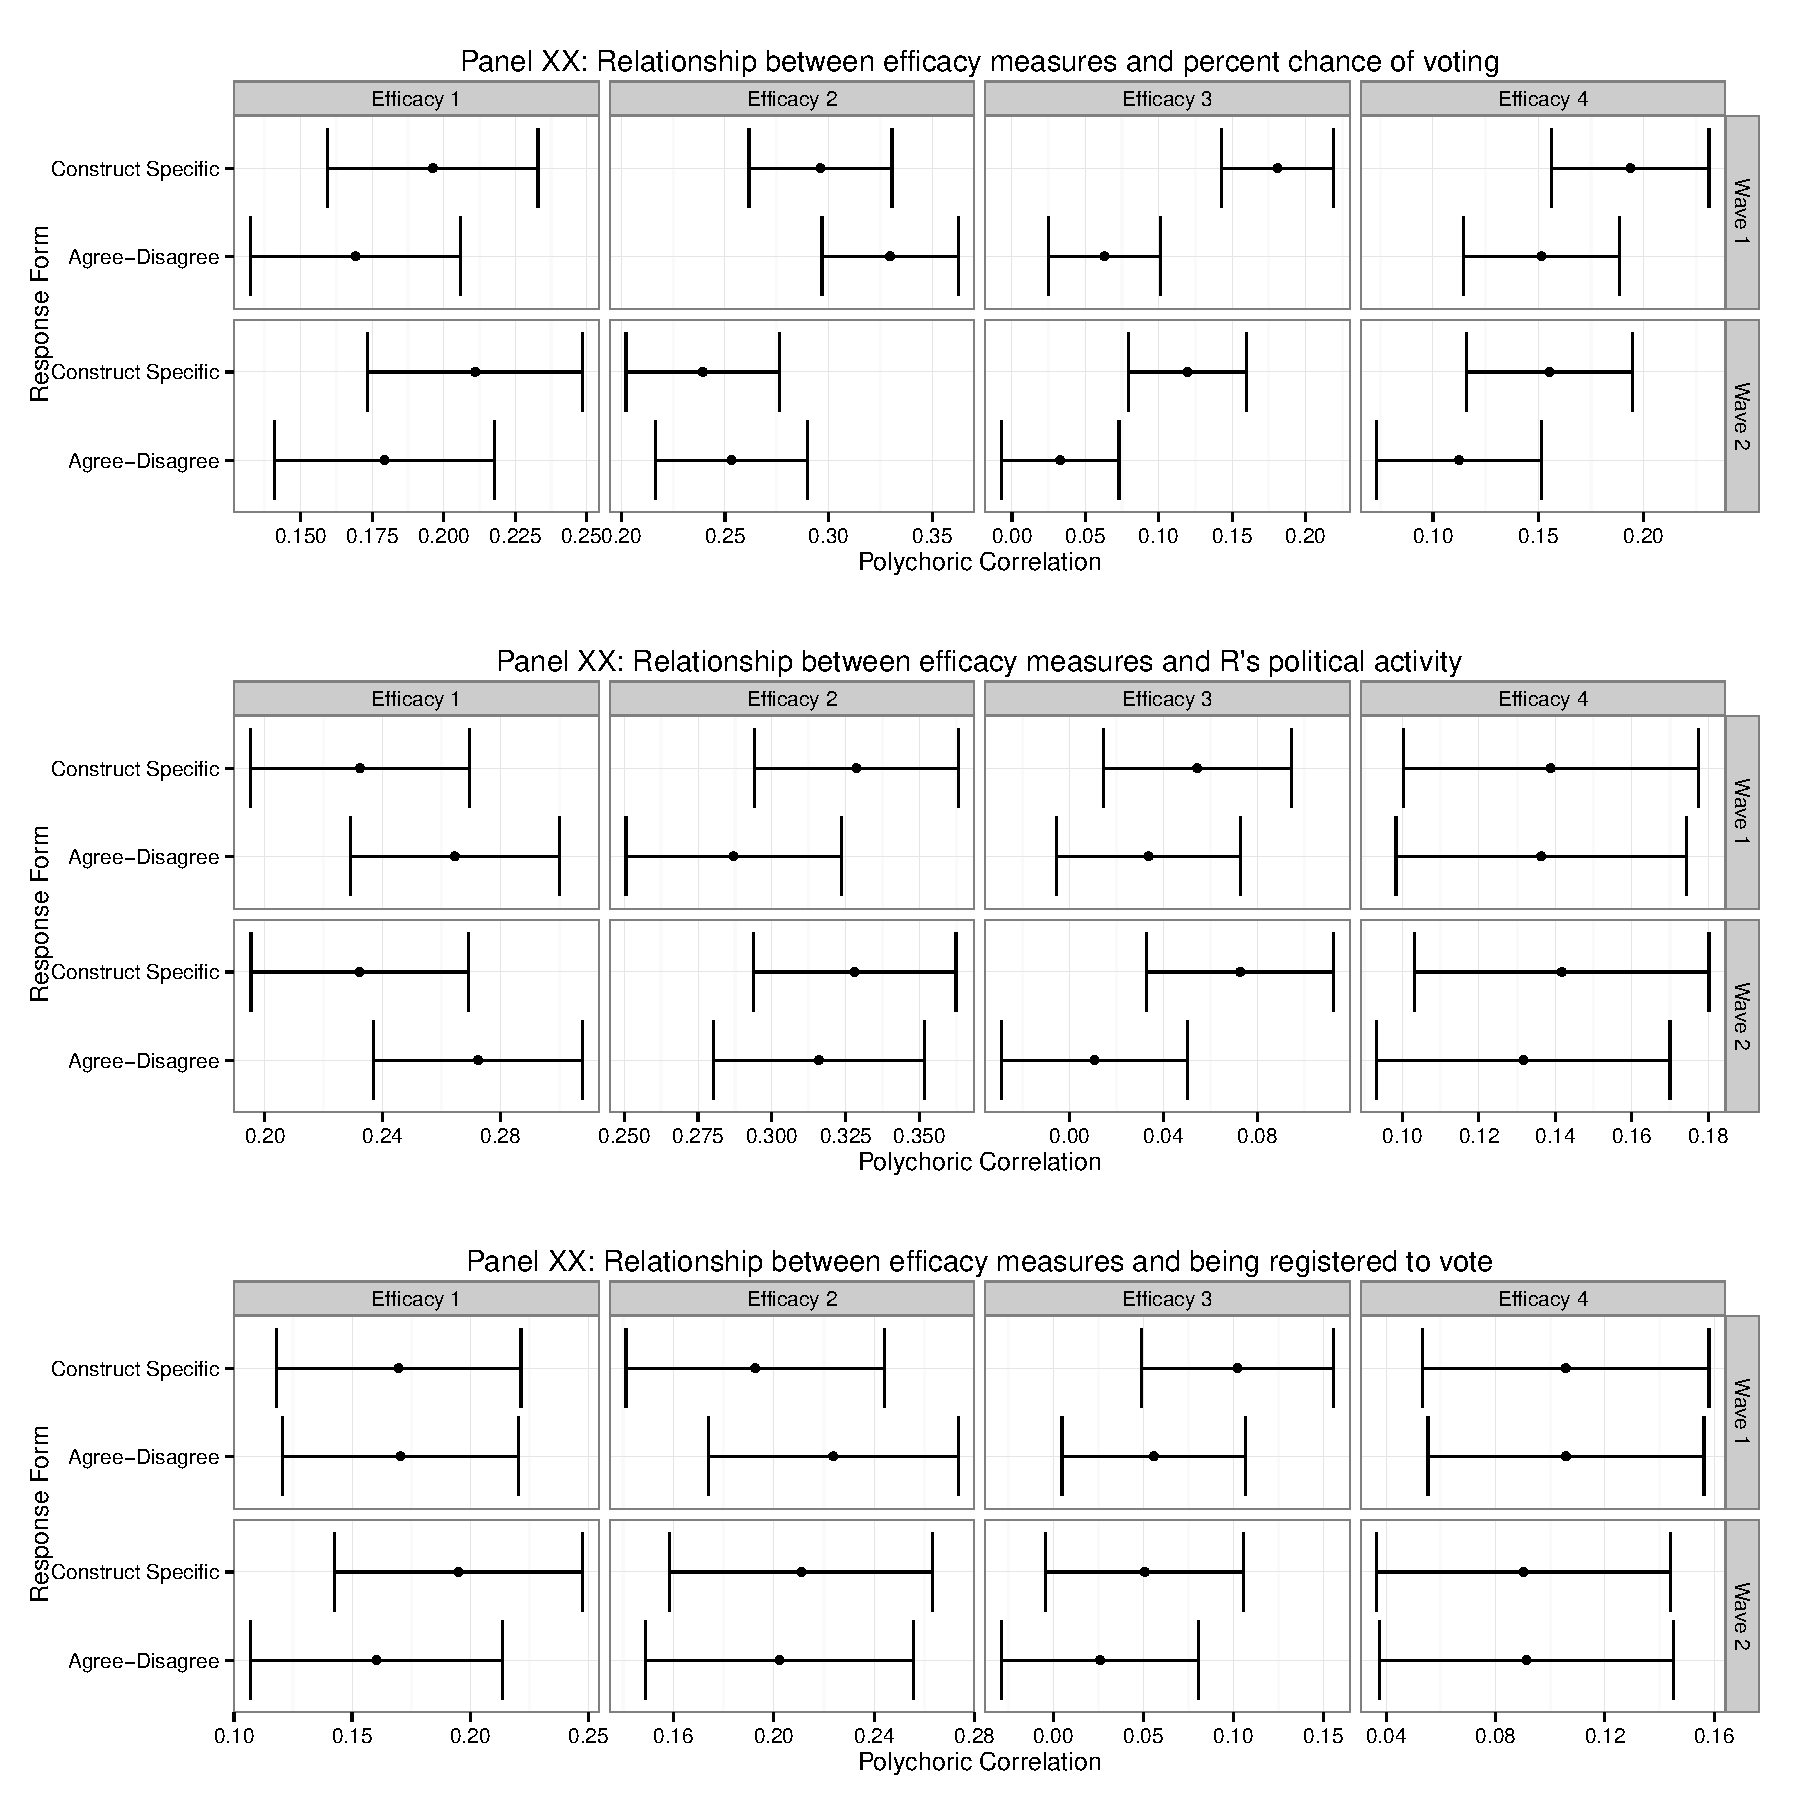
\includegraphics[width=\textwidth]{output/plot1validity.pdf}
\end{figure}

The construct-specific and agree-disagree questions displayed similar levels of criterion validity. The 95 percent confidence intervals around the correlations of the two forms of the question and the percent chance of voting criterion overlapped in all but one case. The construct specific form of the third efficacy measure was more strongly correlated ([.13-.21] in Wave 1; [.11-.19] in Wave 2) with the percent chance of voting question than was the agree-disagree question ([.08-.16] in Wave 1; [.07] in Wave 2). Panel B shows that neither question was more strongly related to respondent's degree of political activism: While the correlations between the agree-disagree questions and the first efficacy measure (in both waves) and political activism were slightly larger than those of the construct-specific measure, the correlations between the second and third construct-specific efficacy measure, on the one hand, and the political activism measure, on the other, were slightly stronger than those of the agree-disagree measure. The correlation between criterion and each of the fourth efficacy measures were almost exactly the same. In all cases, the 95 percent confidence intervals for these correlations overlapped. 

\subsection{Sub-Group Analysis}
\paragraph{Highly Agreeable Respondents}
Respondents that scored in the upper quartile on the agreeableness battery did not consistently give more valid responses when asked about their political efficacy using a construct-specific response scale than when asked about their political efficacy using an agree-disagree response scale (Figure 2).While the point estimates of the correlations between the efficacy measures and the percent chance of voting questions were greater with the construct specific form than the agree-disagree form in 6 of 8 cases (Panel 1, Figure 2), the 95 percent confidence intervals did not overlap in only 2 of the eight cases (in waves 1 and 2 of the Efficacy 3 measure). The average correlation between the agree-disagree scales and the percent chance question was .13; the average correlation between the construct-specific questions and the percent chance question was .19. 

\begin{figure}
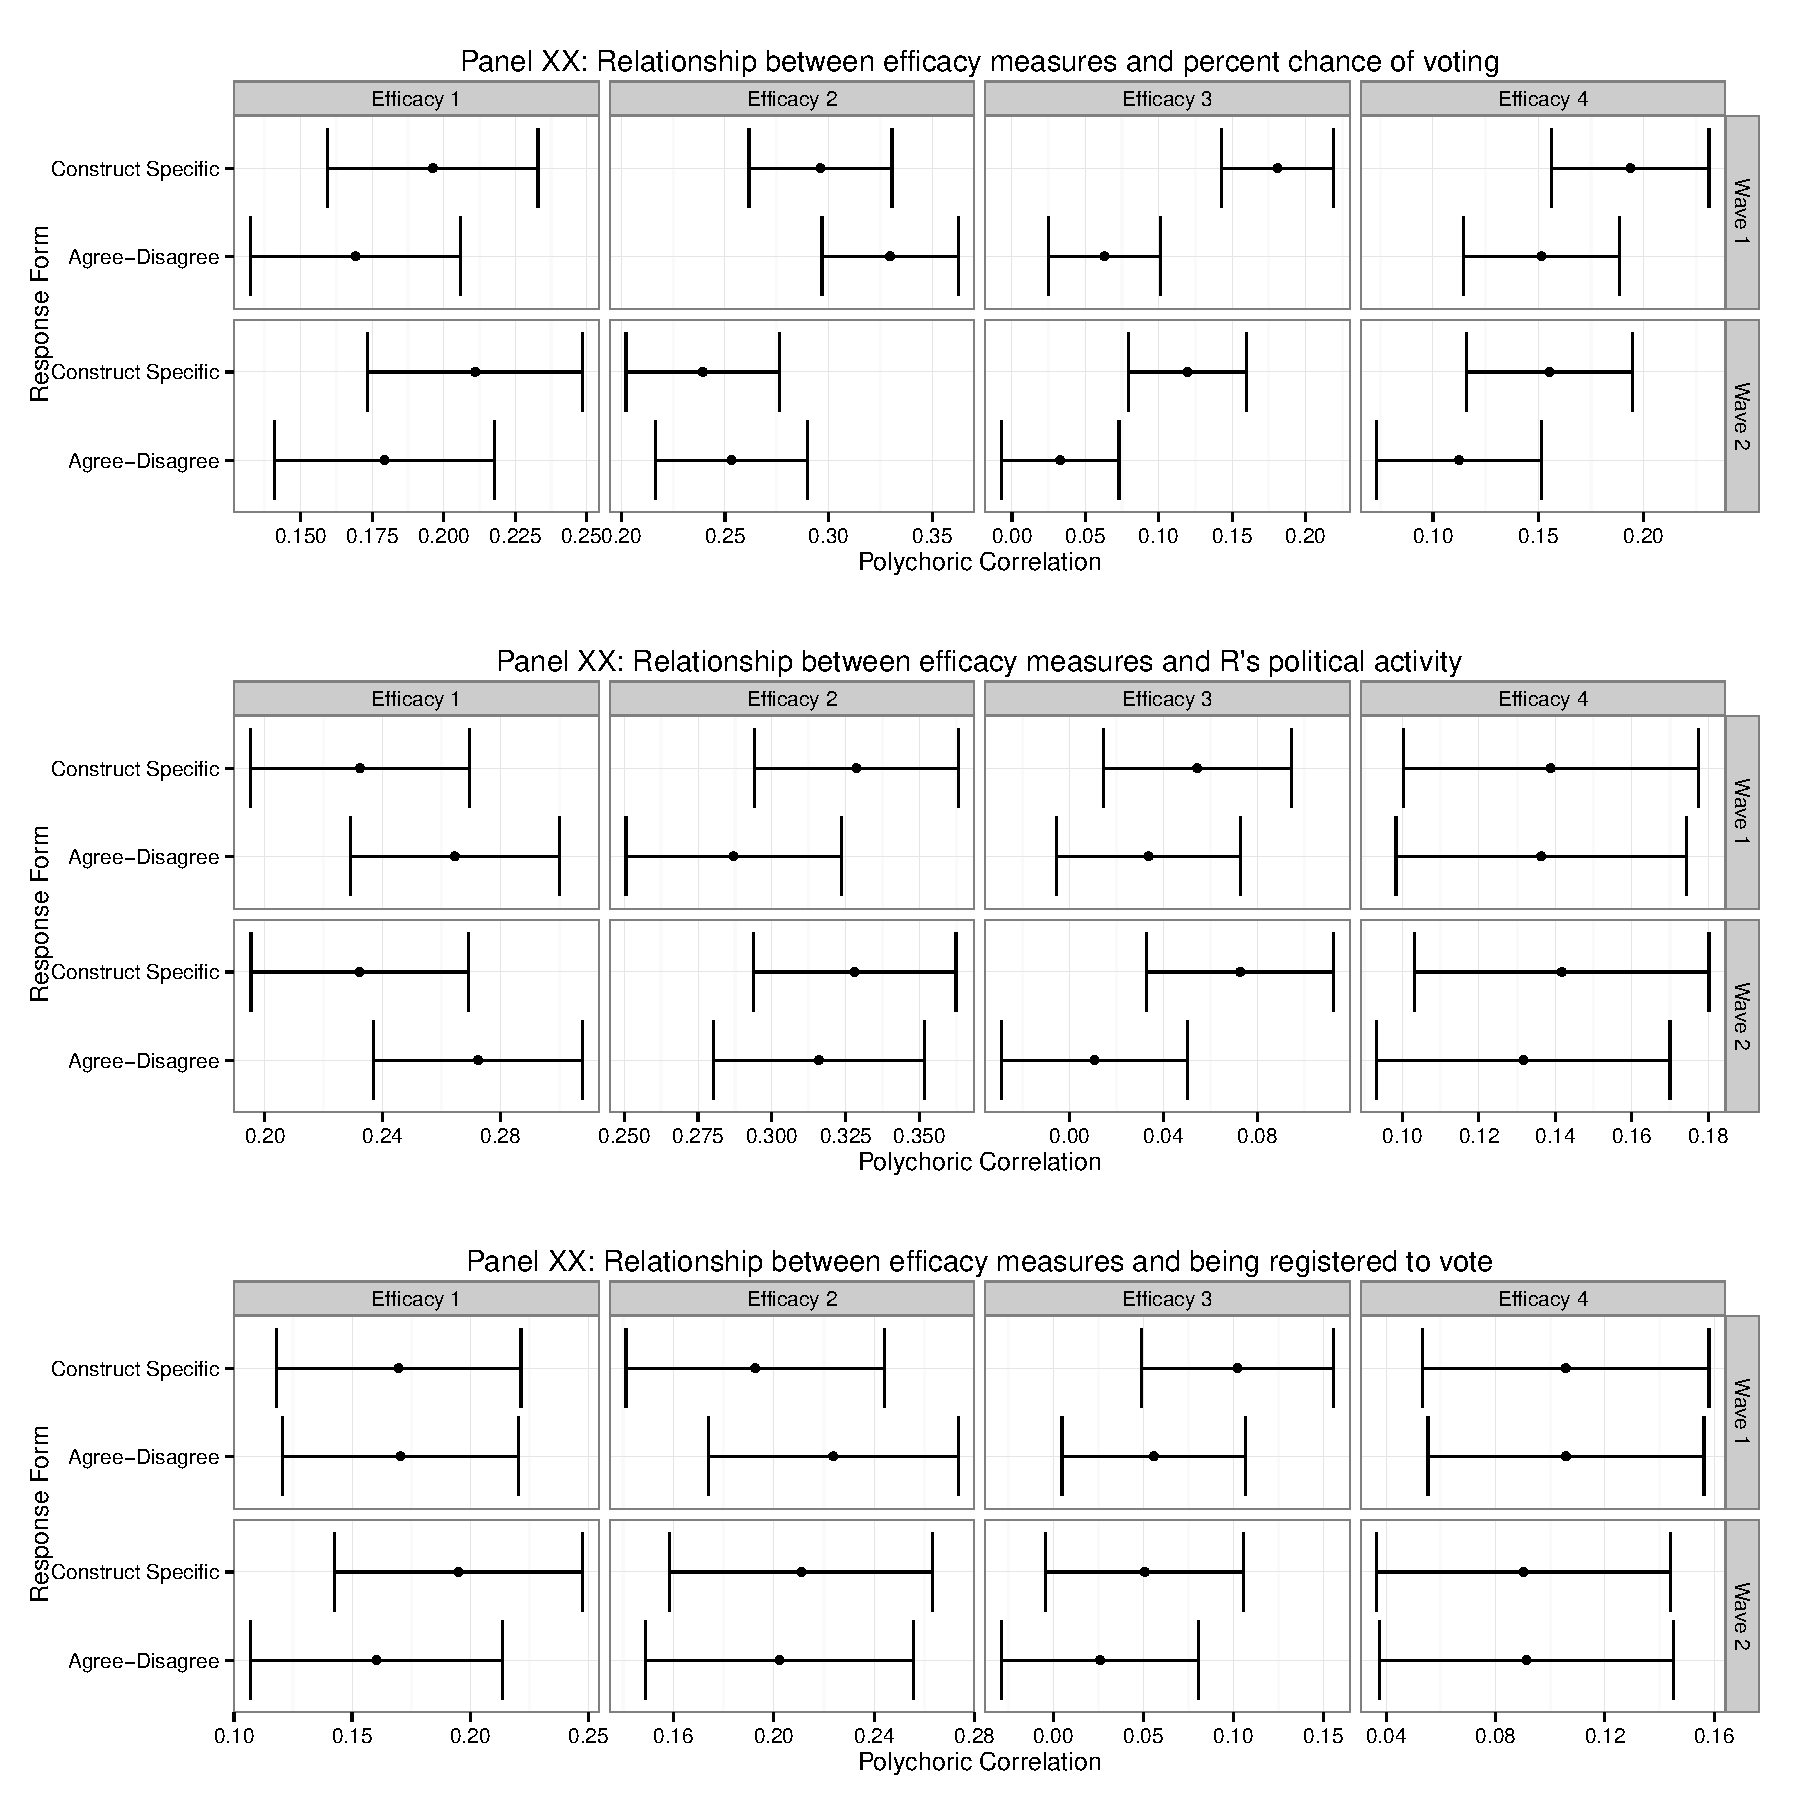
\includegraphics[width=\textwidth]{output/plot2validity.pdf}
\end{figure}

The efficacy questions asked using the construct-specific forms were not more highly associated with the political activity measures than those asked using the agree-disagree forms among highly agreeable people. While the point estimates of the correlations between the of the agree-disagree efficacy questions and the criterion was larger five than the point estimates of the correlations between the construct specific items and the criterion in 5 of 8 cases, the 95 percent confidence intervals overlapped in every case. The average correlation between the agree-disagree questions and the political activity measures were r=.15; the average correlation between the construct-specific form and the political activity measure was r=.17.

Finally, the construct specific questions were also not more closely related to the register-to-vote question than the agree-disagree question among the most agreeable respondents. Although the point estimates of between the construct-specific items and the register-to-vote item in xxx cases, the 95-percent confidence intervals overlapped in each case. The mean correlation between the agree-disagree target and the criterion was .12, while the mean correlation between the construct specific target and the criterion was .16. 

\paragraph{Respondents with low verbal ability}


\begin{figure}
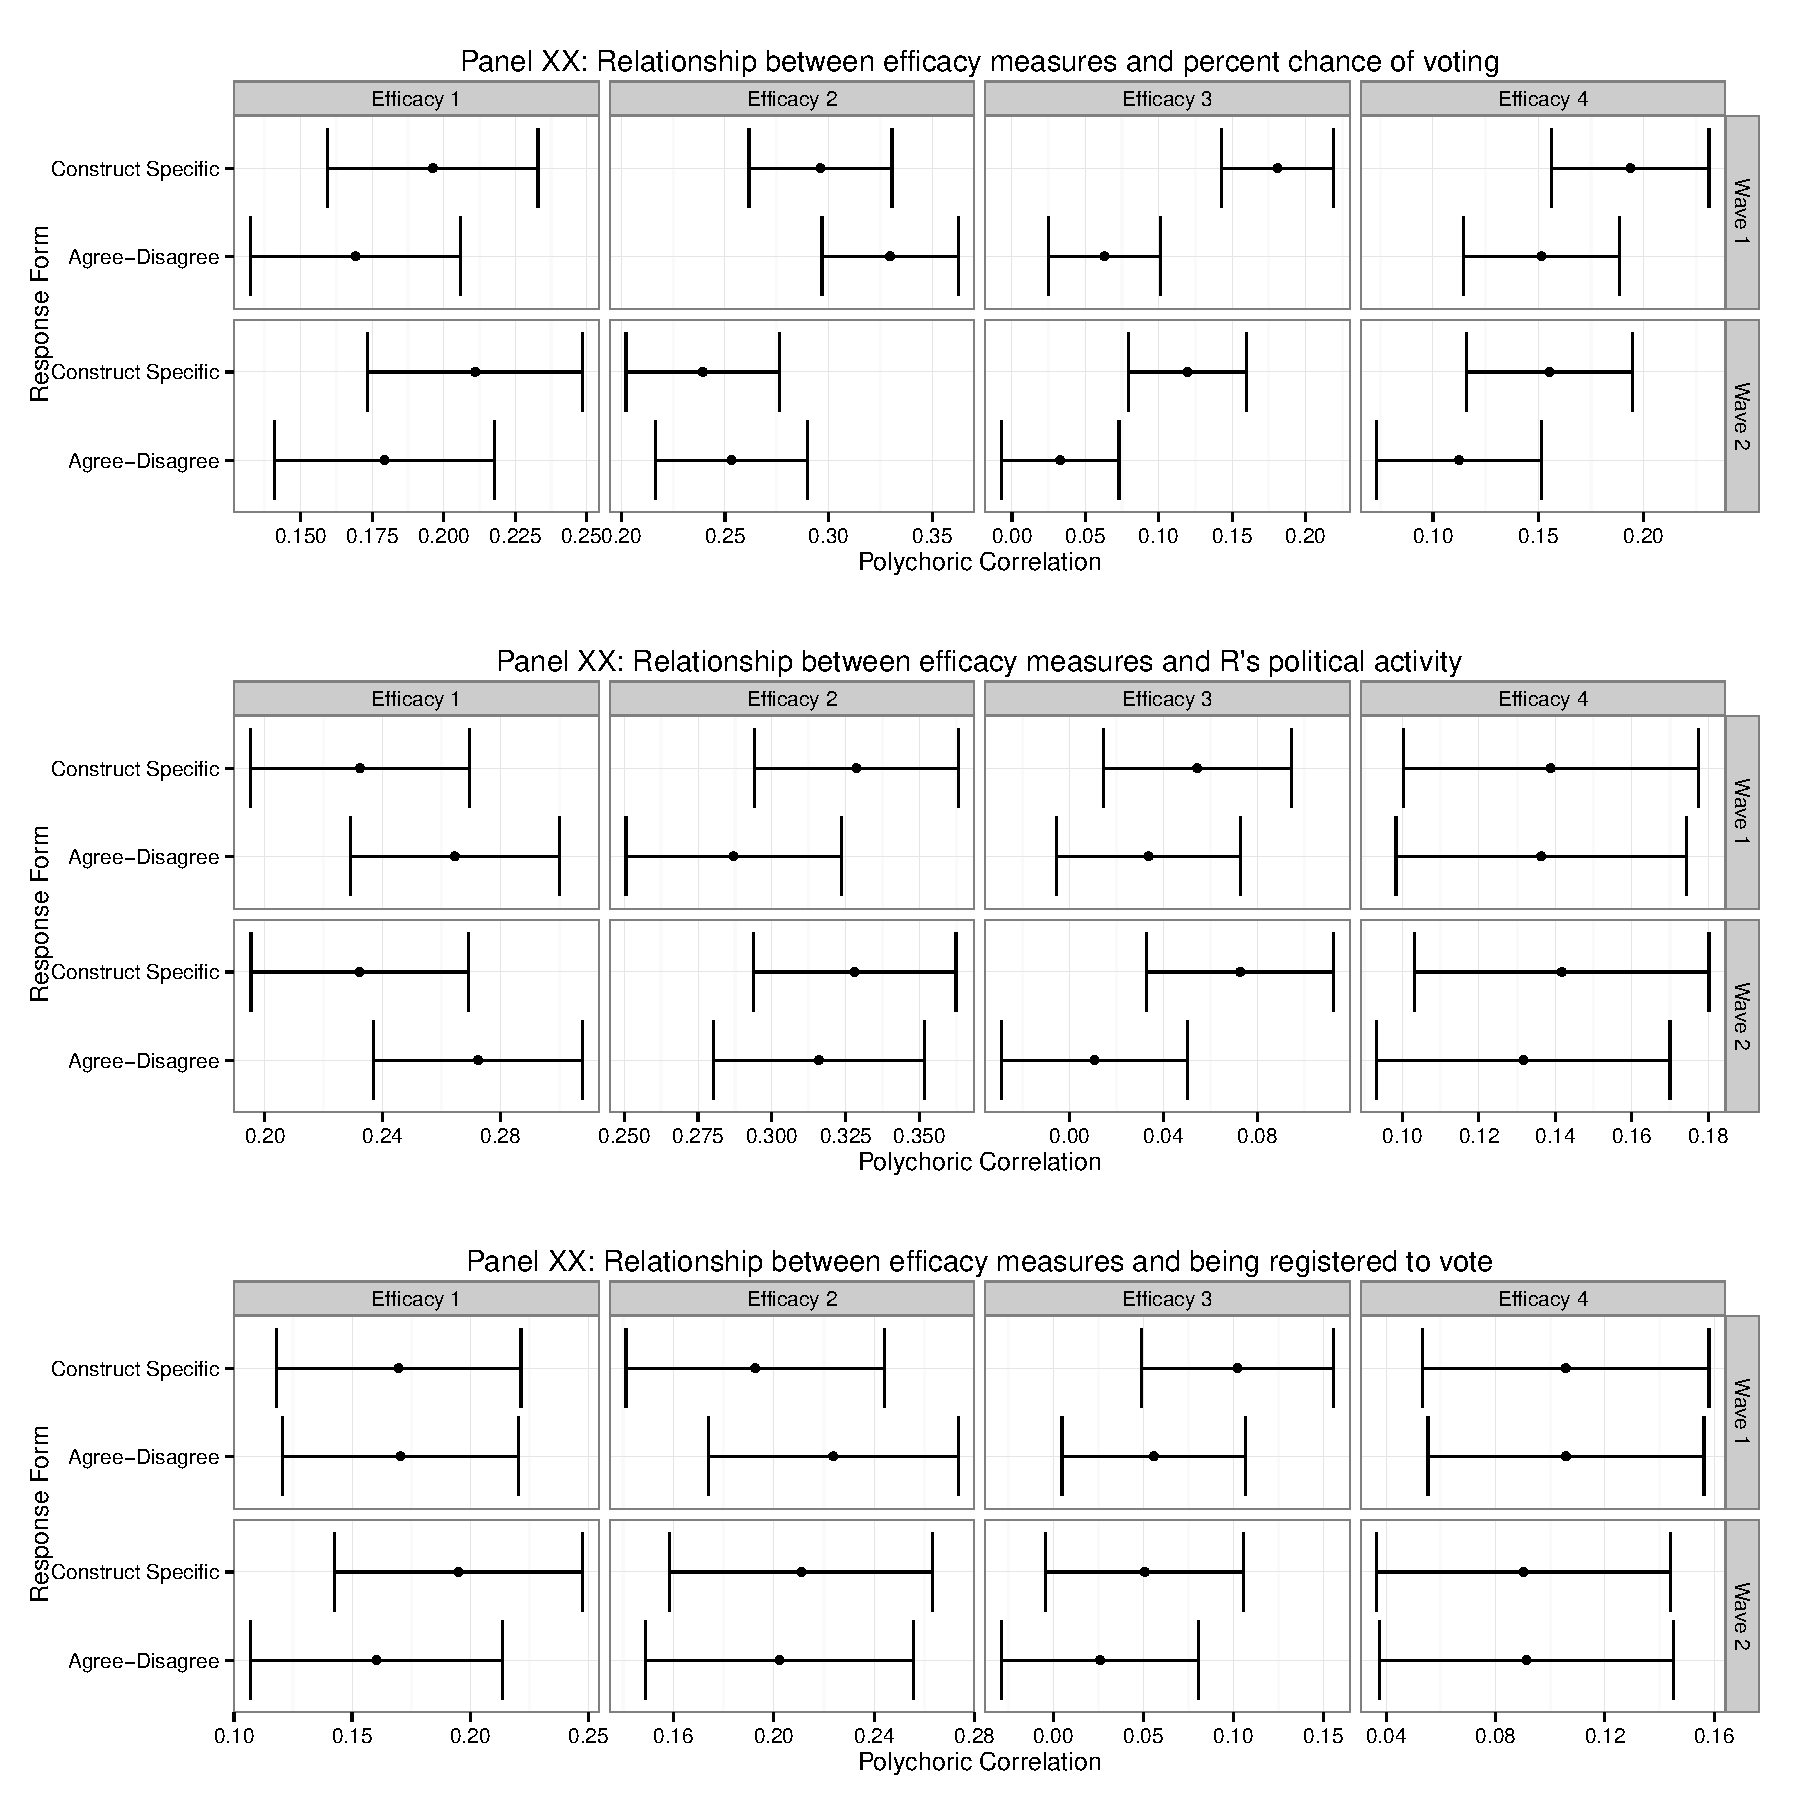
\includegraphics[width=\textwidth]{output/plot2validity.pdf}
\end{figure}

\section{Discussion}

1. reliability not a good indicator, b/c tendency to agree might be stable...
\section{Appendix}

\subsection{Question wording and coding}

\paragraph{Agreeableness}
We￿re interested in how you see yourself. Please mark how well the following pair of words describes you, even if one word describes you better than the other. (Extremely poorly, somewhat poorly, a little poorly, Neither poorly nor well, A little well, Somewhat well, Extremely well):  'critical, quarrelsome' (Reversed Scored); `sympathetic, warm' 

\end{document}
